\nocite{*}

\chapter{Introduzione}

%********************************** %First Section  *************************************
\section{Da dove nasce questo progetto}

Nella carriera universitaria di uno studente è prevista dal piano di studi l'inclusione di un tirocinio (internship) che permetterà allo studente di collaborare con un'azienda in un progetto al di fuori delle mura dell'ateneo. Vi sono due diversi tipi di tirocini, curriculare ed extra-curriculare; il primo permette il riconoscimento di crediti formativi universitari (CFU), mentre il secondo mira solamente a fornire un'esperienza lavorativa allo studente.

Per avviare un tirocinio bisogna quindi mettere in comunicazione soggetti eterogenei, ovvero aziende, professori e studenti. Permettere un'efficace collaborazione tra questi attori che appartengono a categorie e ambienti diversi non è semplice e necessita di un controllo granulare e centralizzato.

Il progetto \projectName~nasce proprio con l'intento di semplificare il processo di gestione degli stage universitari. Il sistema correntemente adottato dall'ateneo non permette un'efficace fruizione dei contenuti né da parte degli studenti né tanto meno dal punto di vista dei professori e delle aziende. L'intero sistema è una semplice interfaccia web che mostra agli studenti autenticati tutte le offerte pubblicate.
%
Il workflow da seguire per inserire, cercare e candidarsi ad un'offerta di tirocinio è piuttosto macchinoso. Se un'azienda desidera proporre un'offerta di tirocinio prima di tutto deve essere convenzionata con l'ateneo, dopodiché deve inviare un'email alla segreteria che provvederà, una volta validato il contenuto dell'offerta, alla pubblicazione della stessa. Una volta pubblicata l'offerta sarà visibile dagli studenti che potranno candidarsi contattando prima il professore e in seguito l'azienda, sempre mediante un rapporto basato su email. 

Risulta quindi necessaria una soluzione che permetta di automatizzare il più possibile questo processo, che tenga traccia dell'andamento del tirocinio e ne monitori lo stato.



%********************************** %Second Section  *************************************
\section{Scelte e vincoli tecnici} 

La soluzione deve essere fruibile da quanti più dispositivi possibili e per raggiungere questo obiettivo ho scelto di sviluppare un'applicazione web. Sfruttando, infatti, l'accessibilità offerta da un applicativo online sarà sufficiente mantenere una sola soluzione per raggiungere tutti i dispositivi più utilizzati --- computer, smartphone e tablet.

Un requisito di fondamentale importanza è quindi un design responsivo dell'applicazione, data la diversità dei dispositivi che si intende supportare. 
Per favorire ulteriormente l'accessibilità dell'applicazione, inoltre, essa dovrà essere multilingua e in questa prima versione supportare almeno l'italiano e l'inglese.

\section{Tecnologie adottate}
Dal momento che ho deciso di puntare su un'applicazione web, le tecnologie che andrò ad utilizzare per il \gls{frontend} della soluzione saranno sicuramente web-based, in particolare lo stack \gls{mean}. Questo insieme applicativo è composto da
\begin{enumerate}
	\item Un \acrshort{dbms} basato su un database documentale \acrshort{nosql} (\mongodb)
	\item Un \gls{framework} server-side per la creazione di applicazioni web e \acrshort{rest} \acrshort{api} (\expressjs)
	\item Un \gls{framework} per la creazione di \acrshort{spa} client-side (\angular)
\end{enumerate}


\subsection{\mongodb}

\mongodb~è un \gls{dbms} non relazionale, orientato ai documenti classificato come \gls{nosql}. Questo significa che rispetto ai tradizionali sistemi relazionali \mongodb~si basa sul concetto di documento e collezione.

Il documento rappresenta un oggetto che si intende memorizzare, mentre una collezione è un insieme di documenti (una tabella se paragonata ai sistemi relazionali).
\mongodb~memorizza i dati in con una rappresentazione binaria chiamata \gls{bson}. Questa codifica estende la popolare rappresentazione \gls{json} per includere tipi di dato addizionali, come \textit{int, long, date, floating point e decimal 128}. I documenti \acrshort{bson} possono contenere uno o più campi, ognuno dei quali contiene il valore di uno specifico tipo di dato, inclusi array, dati binari o sotto-documenti.

\begin{figure}[!h] 
	\centering    
	\lstinputlisting{Chapter1/example.bson}
	\caption[Esempio di paragone \acrshort{json}-\acrshort{bson}]{Esempio di paragone \acrshort{json}-\acrshort{bson}}
	\label{fig:json-bson}
\end{figure}
\noindent
Rispetto a \acrshort{json}, \acrshort{bson} è progettato per essere efficiente sia nello spazio di archiviazione che nella velocità di scansione. Gli elementi in un documento \acrshort{bson} sono preceduti da un campo lunghezza per facilitare la scansione e questo in alcuni casi, quando il documento è piccolo,  porterà \acrshort{bson} ad utilizzare più spazio di \acrshort{json} proprio a causa dei prefissi di lunghezza e degli indici di array espliciti.

% Documenti
I documenti \acrshort{bson} di \mongodb~sono concettualmente allineati alla struttura di un oggetto nei linguaggi di programmazione \acrshort{oop}. Questo rende più semplice e veloce per gli sviluppatori modellare la struttura dati dell'applicazione. Tendono infatti a raggruppare tutti i dati di un record in un unico documento, in opposizione al sistema relazionale tradizionale in cui le informazioni sarebbero distribuite su diverse tabelle. Questa sorta di aggregazione del dato riduce drammaticamente il bisogno di operazioni di \gls{sqljoin} su tabelle diverse, ottenendo performance superiori grazie alla singola lettura per il recupero dell'intero documento desiderato.

I documenti \mongodb~possono variare nella struttura. Ad esempio, tutti i documenti che descrivono i clienti potrebbero contenere l'ID cliente e la data in cui hanno acquistato i nostri prodotti o servizi, ma solo alcuni potrebbero contenere il collegamento ai social media dell'utente o i dati sulla posizione dalla nostra applicazione mobile. I campi possono variare da un documento all'altro; non è necessario dichiarare la struttura dei documenti al sistema --- essi sono auto-descrittivi. Se è necessario aggiungere un nuovo campo a un documento, è possibile crearlo senza influire sugli altri documenti nel sistema.

% Collezioni
Le collezioni sono un insieme di documenti per  definizione \textit{schema-less}, ovvero contengono documenti con tipologie eventualmente diverse (non è considerata una best-practice).

% Query
\mongodb, essendo basato sul modello \acrshort{nosql} non utilizza il linguaggio di interrogazione tipico dei sistemi relazionali, ma ne propone uno proprio.
\begin{figure}[H] 
	\centering    
\lstinputlisting{Chapter1/mongodb.nosql}
	\caption[Esempio di sintassi di \mongodb]{Esempio di sintassi di \mongodb~\textit{vs} SQL}
	\label{fig:mongodb-syntax-example}
\end{figure}

% Table
\noindent
\mongodb~presenta alcune funzionalità non previste dalle altre architetture di database. Una comparazione delle features più interessanti tra \mongodb~e altri tipi di database è raffigurata in tabella \ref{table:mongodbquerymodel}.
\begin{table}[!h]
	\caption{Confronto modello query e indicizzazione di \mongodb~e altri database\cite{mongodbarchitecture}}
	\centering
	\label{table:mongodbquerymodel}
	\begin{tabular}{c c c c}
		  & \mongodb & Database relazionale  & Database Key-value\\ 
		\midrule
		\multicolumn{1}{l}{Query Key-value} & Si & Si  & Si   \\
		\multicolumn{1}{l}{Indici secondari} & Si & Si  & No   \\
		\multicolumn{1}{l}{Intersezione indici} & Si & Si  & No   \\
		\multicolumn{1}{l}{Range queries} & Si & Si  & No   \\
		\multicolumn{1}{l}{Query geospaziali} & Si & Aggiunta costosa  & No   \\
		\multicolumn{1}{l}{Faceted Search} & Si & No  & No   \\
		\multicolumn{1}{l}{Aggregazione e trasformazione} & Si & Si  & No   \\
		\multicolumn{1}{l}{Equi e Nonequi \gls{sqljoin}} & Si & Si  & No   \\
		\multicolumn{1}{l}{Graph processing} & Si & No  & Si   \\
		\bottomrule
	\end{tabular}
\end{table}

\subsection{\nodejs}
\nodejs~è un ambiente open source e cross platform sviluppato a partire dal 2009 che permette di eseguire codice \gls{javascript} lato server.
\begin{quote}
	<<Node.js\textregistered ~ è un runtime \gls{javascript} costruito sul motore \gls{javascript} V8 di Chrome. Node.js usa un modello I/O non bloccante e ad eventi, che lo rende un framework leggero ed efficiente. L'ecosistema dei pacchetti di Node.js, npm, è il più grande ecosistema di librerie open source al mondo.>> \cite{nodejs}
\end{quote}

\noindent
Storicamente \gls{javascript} era utilizzato solamente per scripting client-side, spesso incluso all'interno delle pagine web dove veniva eseguito client-side nel browser dell'utente. \nodejs~permette agli sviluppatori di utilizzare scripting server-side, eseguendo comandi che producono contenuto dinamico prima che venga inviato al browser client-side. \nodejs~rappresenta il paradigma <<\gls{javascript} everywhere>>\cite{jseverywhere}, unificando lo sviluppo di applicazioni web attorno ad un unico linguaggio di programmazione piuttosto che separando i linguaggi per client e server-side.

% Archietettura nodejs
La sua architettura è basata sul modello orientato agli eventi (\acrshort{eda}); ciò significa che \nodejs~richiede al sistema operativo su cui è in esecuzione di ricevere notifiche al verificarsi di determinati eventi, rimanendo in stato di \textit{sleep} fino al ricevimento di tale notifica. Questo pattern architetturale permette una forma di comunicazione non bloccante basata sull'\textit{asynchronous I/O} che per il programmatore finale si traduce nell'utilizzo di \textit{\gls{callback}}. Per segnalare la conclusione di un \textit{task I/O} infatti, \nodejs~invoca la corrispondente \textit{\gls{callback}}, una semplice funzione, alla quale vengono passati i risultati dell'operazione appena conclusa.
%Dettagli tecnici
\nodejs~opera in un processo single-thread utilizzando il pattern \textit{\acrshort{patternobserver}} per la sottoscrizione e la gestione degli eventi, ottenendo così performance adatte ad applicazioni altamente real-time. Processa le richieste in arrivo in un ciclo, chiamato \textit{\gls{eventloop}}, dove ogni connessione è una piccola allocazione di memoria heap anziché un nuovo processo o thread. Alla fine della registrazione della \textit{\gls{callback}} il server rientra in modo automatico nell'\textit{\gls{eventloop}}, a differenza di altri server orientati agli eventi e vi esce solo quando non vi sono ulteriori \textit{\gls{callback}} da eseguire.

% Vantaggi e svantaggi
I vantaggi che hanno portato \nodejs~ad avere una diffusione così ampia sono molti. Sicuramente possiamo notare che \gls{javascript} è un linguaggio ben conosciuto e largamente utilizzato, quindi la curva di apprendimento di questa tecnologia è molto più breve; offrendo inoltre la programmazione orientata agli eventi permette agli sviluppatori di creare server in grado di gestire un alto numero di richieste simultanee che siano facilmente scalabili senza l'utilizzo del \textit{threading}. Lo svantaggio principale di \nodejs~è la mancanza al supporto per la scalabilità verticale, determinata dalla sua architettura single-thread.

\subsection{\expressjs}
\expressjs~è un \textit{\gls{framework}} per costruire applicazioni web ed \textit{\acrshort{api}} basato sulla piattaforma \nodejs. Nel corso del tempo è divenuto lo standard de facto per i \textit{\gls{framework}} server di \nodejs. 
% Descrizione principale
Si presenta in modo minimale, offrendo un sottile livello applicativo che punti a velocizzare lo sviluppo senza tuttavia oscurare le funzionalità di \nodejs. \expressjs~è diviso in diversi moduli che possono essere innestati uno sopra l'altro, rendendolo adatto ad ogni tipo di applicazione.  
% Principali funzionalità
Le sue funzionalità principali sono:
\begin{enumerate}[label=(\alph*)]
	\item Un sistema di routing: contenuto all'interno del pacchetto `express-router`, è il modulo per la gestione e la manipolazione delle routes. Permette di definire in modo gerarchico un insieme di \textit{\acrshort{url}}, alle quali associare una specifica azione. Un'azione è un metodo che viene invocato e che produce una risposta.
	\item \textit{\acrshort{http}} helpers, come redirect o sistemi di caching: contenuto all'interno del modulo core, mette a disposizione alcune utility class che facilitano operazioni ripetitive oppure forniscono strumenti aggiuntivi utili ad ogni tipologia di sistema che si intende sviluppare
	\item Supporto a diversi template engines. Dal momento che si possono anche realizzare applicazioni che ritornano del contenuto, ad esempio un'applicazione \textit{\gls{mvc}}, è necessario un interprete del template che permetta l'inserimento dinamico di contenuto all'interno di esso. Un esempio di quelli che \expressjs~supporta out of the box sono \textit{Pug (Jade), Haml.js, React, Blade} e altri.
\end{enumerate}
% Image
\begin{figure}[!h] 
	\centering    
	\lstinputlisting{Chapter1/express.ts}
	\caption[Esempio di applicazione \expressjs]{Un esempio di applicazione \expressjs}
	\label{fig:expressjs-example}
\end{figure}
Come possiamo vedere in figura \ref{fig:expressjs-example}, una volta creata l'applicazione (riga 3), viene registrata una nuova route (riga 5) alla quale viene associata una \textit{\gls{callback}}. Questa \textit{\gls{callback}} riceve due parametri, la richiesta e la risposta. Il processo di \nodejs~resterà in stato di sleep fino a che una nuova richiesta verrà inoltrata nella route appena definita (quindi fino a che non verrà eseguita una chiamata in \textit{\acrshort{http} GET} all'indirizzo dove è in esecuzione l'applicazione). Una volta ricevuta la notifica \nodejs~entrerà nell'\textit{\gls{eventloop}} per gestirla e una volta completata l'operazione eseguirà la \textit{\gls{callback}} registrata, rispondendo al client che ha effettuato la connessione con la stringa 'Hello World!'.

\subsection{\angular}

\angular~è un \gls{framework} sviluppato da Google per lo sviluppo \gls{frontend} di \gls{spa} basato su \gls{typescript}. Gli elementi costitutivi principali di \angular~verranno discussi nei prossimi paragrafi.


\subsubsection{NgModules}
\label{chap:ngmodules}
Dichiarano un contesto di compilazione per un insieme di componenti dedicato a un dominio dell'applicazione, un flusso di lavoro o un insieme di funzionalità correlate. Un \textit{NgModule} associa i propri componenti al codice relativo, come i servizi, per formare unità funzionali.
% 
Ogni applicazione \angular~--- che in genere contiene più moduli funzionali ---  ha un modulo radice, denominato convenzionalmente \textit{AppModule}, che fornisce il meccanismo di \textit{bootstrap} che avvia l'applicazione.

Come i moduli \gls{javascript}, anche gli \textit{NgModules} possono importare funzionalità da altri \textit{NgModules} e consentire che le proprie funzionalità vengano esportate e utilizzate da altri \textit{NgModules}.
%
L'organizzazione del codice in moduli funzionali distinti aiuta nella gestione dello sviluppo di applicazioni complesse e nella progettazione delle stesse, aumentando la riusabilità del codice. Inoltre, questa tecnica consente di sfruttare il \textit{lazy loading}, ovvero il caricamento dei moduli su richiesta, al fine di ridurre al minimo la quantità di codice che deve essere caricata all'avvio.

\subsubsection{Components}

Ogni applicazione \angular~ha almeno un componente, il \textit{root component}, che connette una gerarchia di componenti con il \acrshort{dom} della pagina. Ogni componente è definito mediante una classe che contiene i dati e la logica dell'applicazione a cui è associato un \textit{template} \acrshort{html} che definisce come i dati devono essere visualizzati.

I \textit{decorators} sono funzioni che modificano le classi \gls{javascript}, in particolare il decoratore \textit{@Component} identifica la classe immediatamente sottostante come un componente \angular, definendo \textit{template} e \textit{metadati} specifici del componente stesso (come le dipendenze).

Il \textit{template} combina \acrshort{html} con un \textit{markup} di \angular~che può modificare gli elementi \acrshort{html} prima che vengano visualizzati.

Le \textit{directives} forniscono logica al componente e il \textit{binding markup} connette i dati dell'applicazione con il \gls{dom}.

Gli \textit{event binding} permettono all'applicazione di rispondere all'input dell'utente aggiornando i dati dell'applicazione, mentre i \textit{property binding} permettono di interpolare valori calcolati dai dati dell'applicazione all'interno del \textit{template} \acrshort{html}.

Prima che un componente venga visualizzato, \angular~valuta le direttive e risolve la sintassi di \textit{binding} nel \textit{template} per modificare gli elementi \acrshort{html} e il \acrshort{dom} a seconda dei dati dell'applicazione e della loro logica. \angular~supporta il \textit{two-way databinding}, che significa che cambiamenti nel \acrshort{dom}, come input dell'utente, possono venire riflettuti all'interno dei dati dell'applicazione, e viceversa.

\subsubsection{Services e dependency injection}
\label{chap:client:services}
Per dati o logica non associati ad una specifica visualizzazione grafica, oppure che si desidera condividere tra componenti, si crea una \textit{service class}. La definizione di un \textit{Service} è immediatamente preceduta dal decoratore \textit{@Injectable}. Il decoratore fornisce i \textit{metadati} che consentono al servizio di essere iniettato nei componenti client come dipendenza.

La \gls{di}  consente di mantenere le classi dei componenti snelle ed efficienti delegando logiche di business ai servizi iniettati.

\subsubsection{Routing}

L'\textit{NgModule} \textit{Router} fornisce un servizio che consente di definire un percorso di navigazione tra i diversi componenti dell'applicazione e visualizzarne le gerarchie.

Il router mappa percorsi simili a \acrshort{url} per componenti anziché per pagine, ovvero quando un utente esegue un'azione, ad esempio facendo clic su un collegamento --- che dovrebbe caricare una nuova pagina nel browser --- il router intercetta il comportamento del browser e mostra o nasconde le gerarchie di componenti definite nel modello di routing.

Se il router determina che lo stato dell'applicazione corrente richiede funzionalità particolari e il modulo che le definisce non è stato caricato, il router può caricare il modulo su richiesta (\textit{lazy loading}).

\begin{figure}[!h] 
	\centering    
	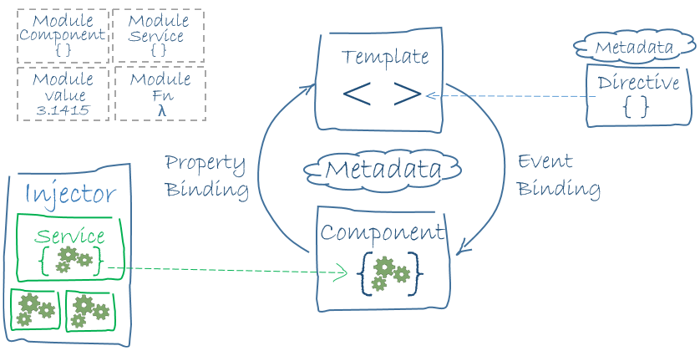
\includegraphics[width=0.8\textwidth]{Chapter1/Figs/angular-overview}
	\caption[Architettura di Angular]{Schema dell'architettura di Angular\cite{angularoverview}}
	\label{fig:angular-overview}
\end{figure}

\section{Attori del sistema}

Dal momento che vi sono più soggetti diversi che accedono alla piattaforma è necessario definire i ruoli dei soggetti coinvolti. Il sistema prevede la gestione di quattro tipi di account --- ognuno con permessi diversi --- e la personalizzazione dell'interfaccia in base all'utente correntemente autenticato. Un account può avere anche più ruoli, ma al momento non ne è previsto l'utilizzo.

\subsection{Azienda}
Rappresenta una (o più) persona fisica responsabile della gestione di un'azienda di cui si fa portavoce.
Deve effettuare l'accesso come un membro esterno dell'ateneo indicando le informazioni della propria azienda e quelle dei suoi amministratori. Inserisce le offerte di tirocinio presso una delle proprie sedi, visualizza le candidature ricevute e approva l'inizio di un tirocinio. Può completare il foglio presenze di un tirocinio in corso nella propria azienda e stamparne la documentazione precompilata al termine. 

\subsection{Professore}
Rappresenta un componente interno all'ateneo che ha il compito di supervisionare le offerte e seguire gli studenti nel percorso.
Deve effettuare l'accesso come un membro dell'ateneo utilizzando l'email istituzionale. Una volta eseguito il login per la prima volta, viene creato un'account il cui ruolo si basa sull'email fornita: se essa termina con \textit{@unive.it} rappresenta un professore, mentre se termina con \textit{@stud.unive.it} rappresenta uno studente. 
Un professore approva le offerte inserite dalle aziende prima che vengano pubblicate, approva e visualizza le richieste di candidatura degli studenti che lo coinvolgono come referente, può completare il foglio presenze di un tirocinio in corso (di cui è referente) e stamparne la documentazione precompilata al termine.

\subsection{Studente}
Rappresenta un componente interno all'ateneo che desidera effettuare un tirocinio in un'azienda.
Deve effettuare l'accesso come un membro dell'ateneo utilizzando l'email istituzionale. Visualizza le offerte di tirocinio pubblicate e propone una candidatura indicando un professore come referente. Può completare il foglio presenze di un suo tirocinio in corso e stamparne la documentazione precompilata al termine.

\subsection{Admin}
Non rappresenta un soggetto fisico, ma bensì una figura che ricopre il ruolo di amministratore dei dati, unico soggetto a non avere restrizioni sulla modifica o la cancellazione di essi. Non ha un'influenza sul processo di gestione dei tirocini in quanto gli altri account formano un ecosistema che si alimenta e gestisce in modo autonomo.